% This file was created by matplotlib2tikz v0.6.18.
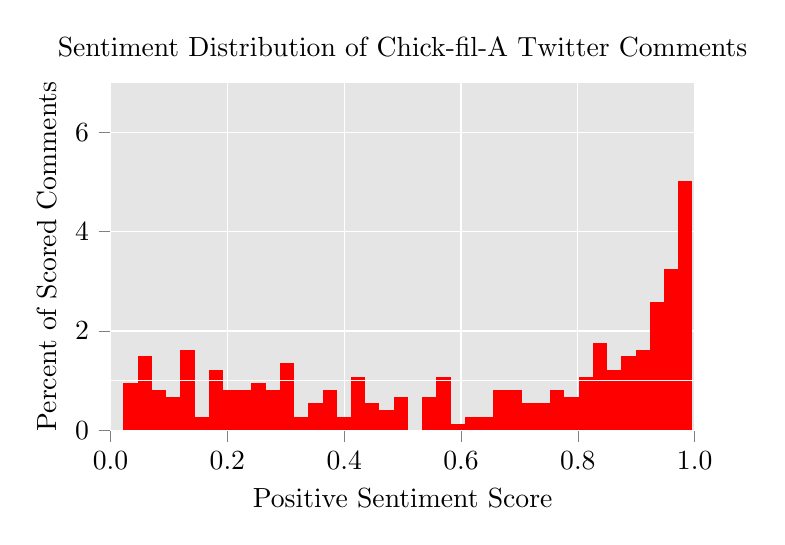
\begin{tikzpicture}

\begin{axis}[
axis background/.style={fill=white!89.80392156862746!black},
axis line style={white},
height=6cm,
tick align=outside,
tick pos=left,
title={Sentiment Distribution of Chick-fil-A Twitter Comments},
width=9cm,
x grid style={white},
xlabel={Positive Sentiment Score},
xmajorgrids,
xmin=0, xmax=1,
xtick={0,0.2,0.4,0.6,0.8,1},
xticklabels={0.0,0.2,0.4,0.6,0.8,1.0},
y grid style={white},
ylabel={Percent of Scored Comments},
ymajorgrids,
ymin=0, ymax=7
]
\draw[fill=red,draw opacity=0] (axis cs:0.0219790190458298,0) rectangle (axis cs:0.0463351532816887,0.948521150382389);
\draw[fill=red,draw opacity=0] (axis cs:0.0463351532816887,0) rectangle (axis cs:0.0706912875175476,1.49053335030431);
\draw[fill=red,draw opacity=0] (axis cs:0.0706912875175476,0) rectangle (axis cs:0.0950474217534065,0.813018191075078);
\draw[fill=red,draw opacity=0] (axis cs:0.0950474292039871,0) rectangle (axis cs:0.119403563439846,0.677515159229232);
\draw[fill=red,draw opacity=0] (axis cs:0.119403563439846,0) rectangle (axis cs:0.143759697675705,1.62603588474317);
\draw[fill=red,draw opacity=0] (axis cs:0.143759697675705,0) rectangle (axis cs:0.168115824460983,0.271006146592908);
\draw[fill=red,draw opacity=0] (axis cs:0.168115824460983,0) rectangle (axis cs:0.192471966147423,1.21952691355738);
\draw[fill=red,draw opacity=0] (axis cs:0.192471966147423,0) rectangle (axis cs:0.216828092932701,0.813018439778725);
\draw[fill=red,draw opacity=0] (axis cs:0.216828107833862,0) rectangle (axis cs:0.241184249520302,0.813017942371583);
\draw[fill=red,draw opacity=0] (axis cs:0.241184234619141,0) rectangle (axis cs:0.265540361404419,0.94852151307518);
\draw[fill=red,draw opacity=0] (axis cs:0.265540361404419,0) rectangle (axis cs:0.289896488189697,0.813018439778725);
\draw[fill=red,draw opacity=0] (axis cs:0.289896488189697,0) rectangle (axis cs:0.314252644777298,1.35502907494175);
\draw[fill=red,draw opacity=0] (axis cs:0.314252644777298,0) rectangle (axis cs:0.338608771562576,0.271006146592908);
\draw[fill=red,draw opacity=0] (axis cs:0.338608771562576,0) rectangle (axis cs:0.362964898347855,0.542012293185817);
\draw[fill=red,draw opacity=0] (axis cs:0.362964898347855,0) rectangle (axis cs:0.387321025133133,0.813018439778725);
\draw[fill=red,draw opacity=0] (axis cs:0.387321054935455,0) rectangle (axis cs:0.411677211523056,0.27100581498835);
\draw[fill=red,draw opacity=0] (axis cs:0.411677181720734,0) rectangle (axis cs:0.436033308506012,1.08402458637163);
\draw[fill=red,draw opacity=0] (axis cs:0.436033308506012,0) rectangle (axis cs:0.46038943529129,0.542012293185817);
\draw[fill=red,draw opacity=0] (axis cs:0.46038943529129,0) rectangle (axis cs:0.484745562076569,0.406509219889363);
\draw[fill=red,draw opacity=0] (axis cs:0.484745562076569,0) rectangle (axis cs:0.509101688861847,0.677515366482271);
\draw[fill=red,draw opacity=0] (axis cs:0.509101688861847,0) rectangle (axis cs:0.533457815647125,0);
\draw[fill=red,draw opacity=0] (axis cs:0.53345787525177,0) rectangle (axis cs:0.557814061641693,0.677513708461508);
\draw[fill=red,draw opacity=0] (axis cs:0.557814002037048,0) rectangle (axis cs:0.582170128822327,1.08402458637163);
\draw[fill=red,draw opacity=0] (axis cs:0.582170128822327,0) rectangle (axis cs:0.606526255607605,0.135503073296454);
\draw[fill=red,draw opacity=0] (axis cs:0.606526255607605,0) rectangle (axis cs:0.630882382392883,0.271006146592908);
\draw[fill=red,draw opacity=0] (axis cs:0.630882382392883,0) rectangle (axis cs:0.655238509178162,0.271006146592908);
\draw[fill=red,draw opacity=0] (axis cs:0.655238509178162,0) rectangle (axis cs:0.67959463596344,0.813018439778725);
\draw[fill=red,draw opacity=0] (axis cs:0.67959463596344,0) rectangle (axis cs:0.703950762748718,0.813018439778725);
\draw[fill=red,draw opacity=0] (axis cs:0.703950762748718,0) rectangle (axis cs:0.728306949138641,0.542010966769206);
\draw[fill=red,draw opacity=0] (axis cs:0.728306949138641,0) rectangle (axis cs:0.75266307592392,0.542012293185817);
\draw[fill=red,draw opacity=0] (axis cs:0.75266307592392,0) rectangle (axis cs:0.777019202709198,0.813018439778725);
\draw[fill=red,draw opacity=0] (axis cs:0.777019202709198,0) rectangle (axis cs:0.801375329494476,0.677515366482271);
\draw[fill=red,draw opacity=0] (axis cs:0.801375329494476,0) rectangle (axis cs:0.825731456279755,1.08402458637163);
\draw[fill=red,draw opacity=0] (axis cs:0.825731456279755,0) rectangle (axis cs:0.850087583065033,1.7615399528539);
\draw[fill=red,draw opacity=0] (axis cs:0.850087583065033,0) rectangle (axis cs:0.874443709850311,1.21952765966809);
\draw[fill=red,draw opacity=0] (axis cs:0.874443709850311,0) rectangle (axis cs:0.89879983663559,1.490533806261);
\draw[fill=red,draw opacity=0] (axis cs:0.898799896240234,0) rectangle (axis cs:0.923156082630157,1.62603290030762);
\draw[fill=red,draw opacity=0] (axis cs:0.923156023025513,0) rectangle (axis cs:0.947512149810791,2.57455839263263);
\draw[fill=red,draw opacity=0] (axis cs:0.947512149810791,0) rectangle (axis cs:0.971868276596069,3.2520737591149);
\draw[fill=red,draw opacity=0] (axis cs:0.971868276596069,0) rectangle (axis cs:0.996224403381348,5.01361371196881);
\path [draw=white, fill opacity=0] (axis cs:0,0)
--(axis cs:0,7);

\path [draw=white, fill opacity=0] (axis cs:1,0)
--(axis cs:1,7);

\path [draw=white, fill opacity=0] (axis cs:0,0)
--(axis cs:1,0);

\path [draw=white, fill opacity=0] (axis cs:0,1)
--(axis cs:1,1);

\end{axis}
\label{chickt}
\end{tikzpicture}